SyVOLT is a user-friendly Eclipse plugin to verify pre-/post- condition
contracts on model transformations specified in the DSLTrans transformation
language. The tool has a number of unique features, outlined below.

\subsection{Push-Button Proving}
Hidden formal methods: providing the transformation and the contract is
sufficient for the tool to automatically provide formal guarantees of correctness. Once the transformation
and the contracts of interest are created, one command will start the property proving process. This process will automatically create
all required artifacts (as detailed in the following section), run the process,
and then provide the results to the user within the Eclipse environment, as seen
in Figure~\ref{fig:output}. This allows the user to continually stay within the
Eclipse environment, which is where he develops the contracts and the model transformations.

\subsection{Based on Symbolic Execution}
We apply the symbolic execution technique classically used for program
verification, to the verification of model transformations. The DSLTrans
transformations and contracts are built upon typed graphs.
Our contract prover is able to reason over these graphs to prove contracts. An
example of this would be in the Families-To-Persons transformation from the ATL
zoo [CITE]. In this transformation, the name for a person in the output graph is
a concatenation of two strings \cgg{instead of ''strings``, should be ''attributes``} from elements in the input graph. Our contract
prover can prove that this concatenation will be valid in all cases.

\begin{figure}
\centering
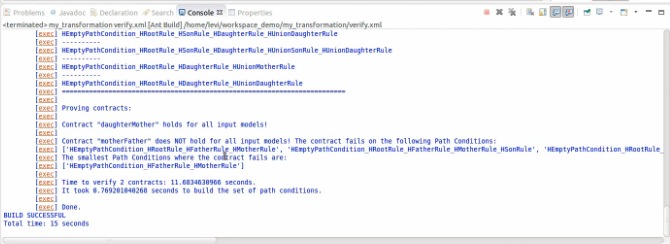
\includegraphics[width=0.45\textwidth]{figures/output}
\caption{The results of the contract prover}
\label{fig:output}
\end{figure}

\subsection{Input Independence and Exhaustiveness}

Our technique will exhaustively prove whether a contract will hold for all
possible input models to a transformation. This allows us to exhaustively verify
a transformation, as seen in~\cite{Lucio2014}.

\subsection{Proving Speed / Scalability}

SyVOLT scales to transformations of practical interest. This has been probed
empirically by applying it to DSLTrans transformations up to X rules, and ATL
transformations up to Y rules. The average size of a DSLTrans transformation is
around XX rules (cite something here) and of ATL rules around YY rules. Even
though our technique is exhaustive, our approach takes a relatively short amount
of time to prove contracts. For example, our experiments on industrial
transformations~\cite{Oakes} show that contracts can be verified within a few
minutes. \cite{Selim2014} demonstrates that our prover is faster than similar
approaches based on SAT solvers. Our approach does not depend on an external
solver and we have implemented the symbolic execution engine from the ground up,
based on model driven techniques, which allowed us to optimize for space and
time economy.

\subsection{Graphical Modelling of Model Transformation Contracts}

Due to the graph-like structure of the pre and post conditions of contracts, the
visual representation of the contract in SyVolt editor allows the user to
quickly build and intuitively understand their meaning.
If a textual (logical or mathematical) editor where to be used, the user would
need an extra system of identifiers to correctly prescribe the structure of contracts.

The visual representation of a contract has all the necessary information to derive the correct 
logical expression to be used by the internal SyVolt prover.

\subsection{Production of Counter-Examples}

When a contract is proved to be violated by a given model transformation, it is useful to also provide an input model - called a \emph{counter-example} - so that the user can execute the model transformation with that input and verify that indeed it violates the contract.

An advantage of out technique is that the counter-example produced by SyVolt
describes a family of input models that violate the contract. This means that
any input model that belongs to the family of the counter-example - i.e., fits
the description given by the contract proving process - causes the model
transformation to violate the contract. \cgg{Levi, did you also show that any
model that does not belong to the family does not cause the model transformation
to violate the contract?} Thus, the user can easily determine the error in the
transformation and correct it. We suggest that this supports a transformation
development method analogous to 'test-driven development'. In this method,
development would be routinely punctuated by contract proof in order to catch
errors early and store test cases - the counter examples produced - to be used in the future.


\subsection{Integration with Eclipse}

Eclipse is a popular development environment and model transformation
tools such as ATL [CITE], DSLTrans [CITE] and EGL [CITE] are integrated with the
Eclipse Modeling Framework (EMF) [CITE].

To take advantage of this ecosystem, SyVolt integrates with EMF.
In the EMF, models can be represented in a multitude of syntaxes, from graphical
to textual, and this makes the interaction with SyVolt easier since the modeler
can use the model editor that is most convenient. Internally, SyVolt uses 
the Himesis format [CITE] to represent models.

\subsection{Model Driven Developed GUI}

To take advantage of the productivity promised by MDD, we used a language called
Eugenia[CITE] to generate the SyVolt contract editor shown in
Figure~\ref{fig:eclipse_frontend}.
With this approach, the SyVolt editor was developed in about 4 man-hours.

\begin{figure}
\centering
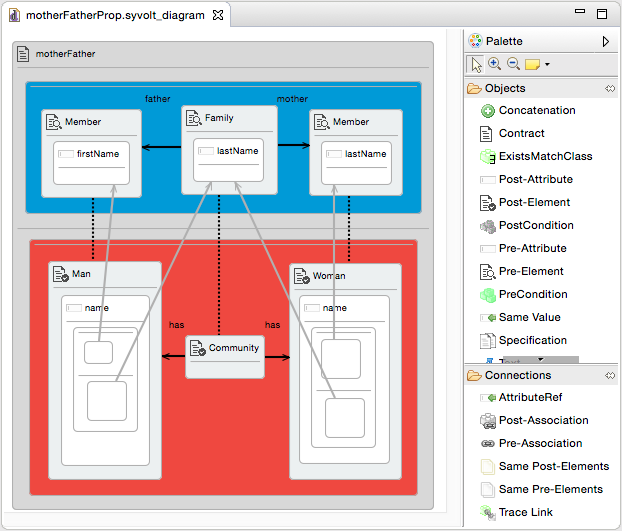
\includegraphics[width=0.45\textwidth]{figures/eclipse_frontend}
\caption{The transformation editor within Eclipse}
\label{fig:eclipse_frontend}
\end{figure}

\subsection{Proving Contracts about ATL Model Transformations}
The Atlas Transformation Language (ATL) is commonly-used in both industry and
academia applications. In order to extend our approach into these domains, we
have developed a higher-order transformation that is able to automatically
transform declarative ATL transformations into our transformation language
DSLTrans~\cite{Oakes}. This allows the user to exhaustively prove contracts on
ATL transformations.


 